\documentclass[border=10pt]{standalone}
\usepackage{tikz}\usepackage{amsmath}\usetikzlibrary{arrows.meta,calc}
\begin{document}
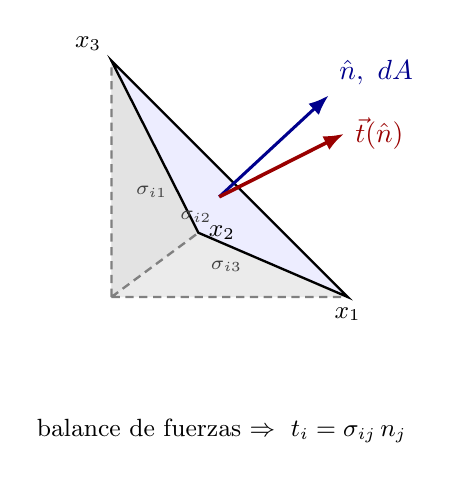
\begin{tikzpicture}[x={(1cm,0cm)},y={(0.46cm,0.34cm)},z={(0cm,1cm)},line width=0.85pt,>={Latex[length=2.6mm]}]
  \coordinate (O) at (0,0,0);
  \coordinate (A) at (3,0,0);   % x1
  \coordinate (B) at (0,2.4,0); % x2 (profundidad)
  \coordinate (C) at (0,0,3);   % x3
  % caras coordenadas (sombreadas) + oblicua
  \fill[black!5]  (O)--(A)--(C)--cycle;
  \fill[black!8]  (O)--(A)--(B)--cycle;
  \fill[black!11] (O)--(B)--(C)--cycle;
  \fill[blue!7]   (A)--(B)--(C)--cycle;
  % aristas: ocultas (a O) discontinuas, oblicua sólida
  \draw[densely dashed,gray] (O)--(A) (O)--(B) (O)--(C);
  \draw (A)--(B)--(C)--cycle;
  \node at (A)[below]{\small$x_1$}; \node at (B)[right]{\small$x_2$}; \node at (C)[above left]{\small$x_3$};
  % normal y traccion sobre la cara oblicua
  \coordinate (G) at (1,0.8,1);
  \draw[->,blue!55!black,line width=1.1pt] (G)--($(G)+(1.0,0.85,1.0)$) node[above right]{$\hat n,\ dA$};
  \draw[->,red!60!black,line width=1.3pt] (G)--($(G)+(1.45,0.3,0.7)$) node[right]{$\vec t(\hat n)$};
  % esfuerzos sobre las caras coordenadas
  \node[black!75] at (1.05,0.05,1.0){\scriptsize$\sigma_{i2}$};
  \node[black!75] at (1.0,1.0,0.05){\scriptsize$\sigma_{i3}$};
  \node[black!75] at (0.05,1.0,1.0){\scriptsize$\sigma_{i1}$};
  \node[align=center] at (1.4,0,-1.7){\small balance de fuerzas $\Rightarrow\ t_i=\sigma_{ij}\,n_j$};
\end{tikzpicture}
\end{document}
